
In this chapter, I show how we extend our layer-based framework to support
verification of a concurrent kernel with fine grained locking.
As illustrated in Chapter \ref{chapter:driver}, our definition of
certified abstraction layers do not directly work with concurrent programs,
as the contextual refinement between the specification and implementation
would not hold due to the arbitrary interleaved executions with other
devices/CPUs. This is because the way we specify the function
does not take account the potential change to the (shared) abstract states
and memory due to the interleavings. On the other hand, it is definitely
not practical to encode all possible ways of the state changes from
interleaved executions in the specifications themselves.

Thus, we need a way to effectively represent the shared states among programs
on different CPUs, and the non-deterministic accesses to these shared
states. Ideally, we would also want to reuse as much framework and techniques
that we have built for verification of sequential programs as possible.
Recall that we have successfully handled some limited form of concurrency
between the devices and a sequential program in Chapter \ref{chapter:driver}.
There, we have developed a new machine model, where the devices are treated
as if they do not execute together with the CPU, and only try to replay
the states of a device when we disable and enable the interrupts on that
device. These two are considered as valid synchronization points because
we do not access the states of the device when the interrupt of the device
is enabled, and we can recompute the current states of the device solely by
applying the device model to the list of external events we observe on that device.

This is clearly restricted to the limited form of concurrency in consideration,
and cannot be directly applied to reasoning of arbitrary concurrent program.
Yet, the general idea is still valid, and we have indeed extended this line of
idea to a concrete framework that is suitable to reason about arbitrary
concurrent programs with fine grained locking in modular ways.
By modular reasoning of concurrent programs, we would expect to reason about
each program running on a CPU or thread separately, by making valid assumptions
to the rest of programs and outside world, and in the end link these individual
proofs formally to reach a final conclusion about the entire program when they
run altogether concurrently. 
In Chapter \ref{chapter:driver}, we still use the abstract states
to model the shared states (the states of devices), which, at synchronization
points, get computed by applying the effect of external events on the current
shared states. Naively applying this would cause the discrepancy when the current
thread uses the abstract states to represent the shares states, while the rest
of the world uses the events. Instead, we always use the list of events to represent
the shared states among threads and processes. In this model, modifying shared
states can be specified simply as appending a new corresponding event to the
event list, and this list can be synchronized by appending the list of events
generated by the rest of the world at every carefully chosen synchronization points.
The the actual shared states can be derived from the list of events by replaying
the effects of the each event in the list from an initial state. We attach such
\emph{replay function} for each shared state and related events.

Recall that in the sequential world, the task of layer based verification is to prove
the contextual refinement between the concrete function implementation manipulating
concrete in-memory data and the abstract high level specification described in
terms of the corresponding abstract states. In this case, the context would be the
user program, other kernel or hypervisor functions, {\it etc}.
In the concurrent world, we also have the programs running on other CPUs/threads,
in parallel with the current function being verified.
Thus, in this case, the task involves proving the contextual refinement between
the function implementation operating on the shared memory and abstract states,
and the abstract high level atomic specification that triggers an atomic high level
event. In the next section, we present this new framework in more detail.

\section{Certified Concurrent Abstraction Layers}

\paragraph{Machine State}
Our new x86 machine state $s$ is a tuple $s~:=~(c, f_p, m, a, l)$.
Here, the component $c$ stands for the current CPU ID, and $f_p$ is
a partial map from a CPU ID to the private states of that CPU.
In addition, $m$ stands for the memory shared across CPUs, and $a$
stands for the shared abstract states. The list $l$ represents
the list of observable global events in the chronological order.
As we mentioned earlier, we represent all shared
states by the list of events, where the concrete states can be reproduced
by applying the replay function to the list of events starting from the initial states.

\paragraph{Transitions}
In the new concurrent machine, a transition may refer to a regular execution
of an assembly instruction, invocation of a private primitive that only changes
CPU local states, or a shared primitive call that could trigger events
observable to other CPUs. To model the non-deterministic execution among
different CPUs, we also have a special transition that changes the current
CPU ID $c$ to some other CPU ID, which we call \emph{hardware scheduling transition}.


\paragraph{Restrictive Memory Model}
Eventually, we would like to prove that every memory access from our entire
verified concurrent program is safe, and there is no data race.
Instead of proving all these desired memory access properties as separate
lemmas for every program, as our usual verification technique, we take a
more systematic approach, i.e., we design a memory model only for safe
memory access such that all the undesired programs semantically get stuck
on our memory model. This ensures that every verified program on our framework
must be data race free.

As a result, in our memory model, we associate every memory block $b$ with
an ownership status in the abstract state $a$, which can only be manipulated
by two new logical abstract primitives \emph{push} and \emph{pull}.
The \emph{pull} operation modifies the ownership status of the memory block
from ``free'' to ``owned by $c$'', while the \emph{push} operation frees back
the ownership of the memory block, together with the updated memory.
These two operations abstract all shared memory access at our
lowest machine model as atomic logical primitives that triggers corresponding
\emph{push} and \emph{pull} events. 
As described above, if a program tries to pull a non-free location, or tries to
access or push to a location that is not owned by the current CPU, the
machine semantics gets stuck. 
This way, we encapsulate every valid shared memory access with corresponding
\emph{push} and \emph{pull} events from involved CPUs.
We show in Section \ref{veri-ticket-lock}
how we can further encapsulate and abstract these logical primitives to
build a spinlock module.


\paragraph{Active CPU Set and Environmental Context}
To enable modular reasoning of concurrent programs, we would like a way
to semantically reason about only part of the whole program locally, by
making reasonable assumptions on the rest of programs, and finally formally
combine the reasoning of these individual programs together, to reach a
final conclusion about the full program.
We call the set of CPUs in consideration the \emph{active CPU set} $A$, and
specify the assumptions over the external world outside $A$ as the
environmental context $\oracle$, which is a partial map from a list of
current global event log $l$ to another list of events $l'$ that corresponds
to the list of observable events triggered by the CPUs outside $A$ at this
interleaving point. We denote such concurrent layer interface $L$ parameterized by
an active CPU set $A$ and environmental context $\oracle$ as
$\PLayer{L}{A}{\oracle}$.

We encode our assumptions on the external world by
enforcing a \emph{Rely} condition on the list of event logs
the environmental context returns,
and represent our own invariants by introducing a \emph{Guarantee} condition
on the list of events triggered by programs running on the active CPU set $A$.
If we have separately verified two sets of concurrent programs running on
a disjoint sets of CPUs $A$ and $B$, and each of the \emph{Guarantee} condition
implies the other's \emph{Rely} condition, then we can merge these two proofs
together to derive a proof on a combined concurrent program running on the
active CPU set $S_{AB}=A\cup B$ and the environmental context 
$\oracle_{AB}=\oracle_A\cap\oracle_B$.
Since the event list $l$ is part of our abstract state, and the list of events
from the environmental context is also appended to $l$, both the \emph{Rely}
and \emph{Guarantee} condition can be represented as regular layer invariants
in our concurrent certified abstraction layer framework.

\ignore{
\paragraph{Concurrent Layer Interface}

Now we define the \emph{concurrent layer interface} $\PLayer{L}{A}{\oracle}$,
parameterized over the active CPU set $A$, and the environmental context
$\oracle$, as a tuple $(\Layer, \Rely, \Guard)$, where the $\Layer$ defines
the abstract states and primitives (similar to the sequential version),
and $\Rely$ and $\Guard$ being the \emph{Rely} and \emph{Guarantee} condition.
}

\paragraph{Building Concurrent Certified Abstraction Layers}
Now we define the contextual refinement in the concurrent setting,
using the definition in the sequential case.

\begin{definition}[Contextual Refinement]
For every code module $M$, active CPU set $A$, and environmental context
$\oracle$, we say $\llbracket{}M\rrbracket{}L_1$ contextually refines
$L_2$ over $A$ and $\oracle$ if and only if there exists a function
$f$ such that $\llbracket{}M\rrbracket{}\PLayer{L_1}{A}{\oracle}$ contextually
refines $\PLayer{L_2}{A}{f(\oracle)}$. 
\end{definition}

Similar to the sequential case, we have developed some proof patterns on
building concurrent certified abstraction layers, layer by layer.
Our verification is still per function basis, and we verify the programs
running on each CPU separately, and build up the standard layer hierarchy
$\PLayer{L}{\{c\}}{\oracle}$ for each CPU $c$. For simplicity, we note this
\emph{CPU local layer} as $\PLayer{L}{c}{\oracle}$.
In the end, we compose these proofs for each CPU
into a combined proof for the whole concurrent program.

We have developed two proof patterns to help building certified concurrent
abstraction layers. First, we use \emph{fun-lift} pattern to abstract shared
physical memory into shared abstract states, and specify and verify the
concurrent functions with these abstract states, in a way very similar to
how we build the sequential layers. Note that this process does not change
any potentially interleavings in the programming executions, and each shared
operation is specified by querying the environmental context to obtain the
external event list at every interleaving point, i.e., our primitive specifications
are no longer atomic as their behavior depends on other concurrent programs' behavior
in the middle of the primitive executions. On the other hand, by not handling
the concurrency at this level allows us to be able to reuse most of the
frameworks and techniques we have built for verifying sequential programs.

Once we are at a layer where we have a full behavior of the shared
``atomic'' primitives, we utilize the second \emph{log-lift} pattern to
lift the layer into a new layer where the specifications of the shared
primitives are atomic, i.e., they simply trigger a new single atomic
event. Proving the contextual refinement between these two layers include
the critical concurrency reasoning on the fact that the events can be
shuffled and merged into a new list where we can always map a consecutive
list of underlay events into a single new event at the overlay.
Concretely, we need to find a function $f$ that can transform the environmental
contextual of underlay into one at overlay, and a refinement relation $R$
that matches the underlay and overlay states, especially the two event list
with events generated both locally and returned by the environmental context.
We illustrate this process in more details in the examples in subsequent sections.

\paragraph{Multicore Linking Theorem.}
By composing all the CPUs in the machine (denoted as the set $D$), the resulting 
layer interface does not depend on any environmental events except those
hardware scheduling transitions among different CPUs.
We construct such a layer interface $\PBoot[D]$
using the primitives provided by the layer $\Mach_{\boot}$, which is the lowest
layer that we use to model the multicore hardware environment. 
We can then prove a contextual refinement from  $\Mach_{\boot}$ to $\PBoot[D]$
for every possible interleaved executions.
\begin{theorem}[Multicore Linking]
\label{thm:link}
$\forall P, \sem{\Mach_{\boot}}{P} \refines_R \sem{\PBoot[D]}{P}$
\end{theorem}
This theorem ensures that all code verification over $\PBoot[D]$ can be propagated down to the x86 multicore hardware 
$\Mach_{\boot}$.


\section{Verification of Ticket Lock}
\label{veri-ticket-lock}


\subsection{Spinlocks}
\begin{figure}[t]
\lstinputlisting [language = C] {src/ticket_lock.c}
\caption{Pseudocode of ticket lock implementation.}
\label{fig:exp:real_ticket_lock}
\end{figure}

Spinlocks are one of the most basic synchronization
methods for multicore machines; they are used as building
blocks for shared objects and more sophisticated synchronizations.


A spinlock enforces mutual exclusion by restricting CPU access to
a memory location $b$. Lock operations can be viewed
as ``safe'' versions of $\push/\pull$ primitives.
For example, when the lock acquire  for $b$ succeeds,
the corresponding shared memory is guaranteed
to be ``clean'', meaning that it is safe to 
pull the contents to the local copy at this point.
As an example, Fig.~\ref{fig:exp:real_ticket_lock} shows
an implementation of the ticket lock algorithm \cite{mcs91}.
As can be seen in Fig.~\ref{fig:exp:real_ticket_lock},
the $\acq/\rel$ functions invoke the $\push/\pull$ primitives.
\footnote{Note that even though these primitives are
called in the layer as if they are actual function primitives,
those are only logical primitives that do not intend to incur
any performance overhead, and are only used as a verification
technique.}
We now show how we build concurrent certified abstraction layers
for the ticket lock implementation shown
in Fig.~\ref{fig:exp:real_ticket_lock}.

\noindent\textbf{Step 1 (memory operation interface $L_0$).}
We first develop a layer, where the three tick related primitives
are abstracted into three atomic primitives \texttt{get\_n},
\texttt{inc\_t}, and \texttt{inc\_n}, which generate corresponding
external low level event. Thus, including the events generated by the
\texttt{push} and \texttt{pull} primitives, the external event list
$l$ in the new layer $L_0$ contains the following sets of events:

\[
\begin{array}{c}
\incticket(b) \mid \incnow(b) \mid \getnow(b)
\mid \push(b,bl) \mid \pull(b)
\end{array}
\] 

To reconstruct the value of $t$ and $n$ from events, we define a replay
function $\replay_{\comm{ticket}} : Log \to \integer \to \integer\times \integer$. 
The definition is as one would expect:
$\replay_{\comm{ticket}}(\mathsf{nil}, b) = (0,0)$, and each 
$\incticket(b)$ and $\incnow(b)$ event in the list increments
the first or second component of the pair, and other events are ignored.

The atomic ticket primitives are implemented using the atomic x86 assembly
instructions. For example, we implement the
fetch-and-increment $\mathsf{FAI\_ticket}$ primitive in a small 
assembly snippet, yielding the following specification:

\begin{mathpar}
\inferrule{
 l_0 = l \cons \oracle(l) \\
  \replay_{\comm{ticket}}(l_0, b) = (i,j) \\
  l' = l_0 \cons c.\incticket(b)\\ 
}{
 \oracle, c \vdash  \spec_{\mathsf{FAI\_ticket}}([b], l, i, l')
}
\end{mathpar}

Here, $c.\incticket(b)$ means the event is triggered by the CPU
$c$, and ``$\cons$'' means ``cons-ing'' an event to the log.
The specification $\oracle, c \vdash  \spec_{\mathsf{FAI\_ticket}}([b], l, i, l')$
indicates that the for all possible environmental context $\oracle$ and
CPU ID $c$, the primitives takes an argument $b$ and returns an
integer $i$, transitioning the event log from $l$ to $l'$. Other
irrelevant states are not shown here for simplicity as they do not change
during this transition.

As shown in the specification,
the primitive queries $\oracle$ and appends the result list and
one new event to the log,
then returns the current state $i$ of {\tt ticket} computed by
replaying the result log.
The fact that we are
using an atomic memory instruction, and that such memory updates are
immediately visible to all CPUs, is reflected by the
primitive just adding a single event so there can be no unexpected
interleavings between CPUs. We add similar specifications for the
other operations, \eg, a $\sigma_{\mathsf{get\_now}}$ primitive whose
implementation is a memory read, and whose specification queries
$\oracle$ to get the new log $l_0$, appends $\getnow (b)$, and returns
$\mathsf{snd}(\replay_\mathsf{ticket}(l_0, b))$.
The layer interface $L_0$ is defined as below:

\[
\begin{array}{rl}
L_0 := &\mathsf{FAI\_ticket} \mapsto \spec_{\mathsf{FAI\_ticket}}
\oplus \mathsf{inc\_now} \mapsto \spec_{\mathsf{inc\_now}} \\
&\oplus \mathsf{get\_now} \mapsto \spec_{\mathsf{get\_now}}\oplus  \push\mapsto \spec_{\push}
\oplus  \pull\mapsto \spec_{\pull}
\end{array}
\]

\noindent\textbf{Step 2 (low-level specification $L_1$)}
Next, following the \emph{fun-lift} pattern,
we verify the implementation of the ticket lock shown in 
Fig.~\ref{fig:exp:real_ticket_lock}, on top of the previous
layer interface $L_0$.
As illustrated before, on this pattern, we do not aim to change
any potentially interleavings in the programming executions, and
we specify each shared operation by querying the environmental context
to obtain the external event list at every interleaving point.
To come up with such a specification at $L_1$ for $\rel$ is
straightforward, and it just appends the $\push$ and $\incnow$ events
to the log, while querying $\oracle$ and appending the result
list before it pushes each event to the log, capturing all possible
interleaved executions at each such synchronization point.

However, we need some care to assign a good specification to
$\acq$, as it contains a while-loop. To prove total correctness,
we would like to assign a specification which later can be proven
to terminate.
We define an auxiliary function $\comm{wait}$
(using recursion in Coq) describing the behavior of the first $k$
iterations of the loop: each time we query the environment
context $\oracle$, it generates its own
event, and checks if CPU number $c$ is due to hold the
lock. The function is undefined (Coq {\tt None}) if we do not get the
lock within $k$ iterations.

\[
\begin{array}{lcl}
\mathsf{wait}(0, \oracle, c, b, l) & = &\text{undefined} \\
\mathsf{wait}(k+1, \oracle, c, b, l) & = & l', \text{ if $l'$ indicates next is $c$'s turn to get lock}\\
                       & &   \mathsf{wait}(k, \oracle, c,  (l' \cons c.\getnow(b))), \text{ otherwise} \\
                       & &  \text{where }l' = l \cons  \oracle(l)
\end{array}
\]

We then define the semantics of the primitive by saying that it first
generates an $\incticket$ event, and then loops
for some ``sufficiently'' large number $\calwait(l, c)$ of iterations.

\begin{mathpar}
\inferrule{
  l_0 = \mathsf{wait}(\calwait(l, c), \oracle, c, b,
  	l \cons \oracle(l) \cons c.\incticket(b)) \\
  	l'  = l_0 \cons c.\pull(b) \\
}{
 \oracle, c \vdash  \spec_{\acq\_\mathsf{low}}([b], l, \any, l')
}
\end{mathpar}

Computations where $k$ reaches 0 are considered stuck, and our
ultimate theorem is about safe programs (programs that does not get stuck).
Thus, to prove the \textbf{starvation-freedom} of ticket lock,
we have to know what number $\calwait(l,c)$ is sufficiently large.
We make following two assumptions. Fist, the hardware scheduling transition
is fair, i.e., there exists a number $h$ such that the nondeterministic execution is
guaranteed to get back to the previous CPU within $h$ hardware steps.
Second, every CPU who acquired the ticket lock released the lock within
$r$ steps for some constant $r$. This is also a reasonable assumption because if someone
holding the lock never releases the lock, no one else can ever obtain the lock
again. Both of these assumptions are formally enforced by introducing
them as layer invariants on the event list $l$.
Given these two assumptions, and also assuming there are $n$ number
of CPUs available on the machine, we can conclude that each CPU
needs to wait on the lock for at most $h * r * n$ steps, as even if all
other CPUs were in the queue ahead of the current CPU, they would eventually
all release the lock within these many steps and no one can take the lock
bypassing the currently CPU's turn by definition of the ticket lock.

The main task in proving the contextual refinement between $L_1$ and $L_0$
is to prove that the implementation shown in Fig.~\ref{fig:exp:real_ticket_lock}
satisfies the specifications shown above. The refinement proof is
straightforward because the abstract state and the global log are identical
in both layers, and thus the simulation relation is the identity relation.

On the other hand, in this \emph{fun-lift} pattern, we can reuse all the
techniques we have developed for verification of sequential programs, as
there is no reasoning of interleavings involved here. One technical challenge
apart of concurrency is that the ticket in the specification increases
monotonically, while in the implementation, we have to use finite precision
integers that wraps back to zero when it reaches the maximum. Thus, as you
see in the implementation, we use the $!=$ operator instead of $<=$.

\vspace{3pt}
\noindent\textbf{Step 3 (atomic specification $L_2$)}
Recall that the specification $\spec_{\acq}$ and $\spec_{\rel}$ in $L_1$
are not atomic, as they involve potential interleavings in the middle
(encoded by querying the environmental oracle for external events).
On the other hand, as clients using the lock, we would treat the lock
primitives as if they were atomic, even in reality, there could be
some irrelevant interleaved executions in the middle.
We achieve this by introducing a new higher layer interface $L_3$ using
the \emph{log-lift} pattern, which contains atomic specifications
for $\acq$ and $\rel$ primitives.

Unlike previous two layers, the new layer $L_3$ does not contain any of
the low level events, but instead contains two new events
$\acq(b)$ and $\rel(b)$. The specifications for the two primitives are
now very simple: they just query the environment context, and then
introduce one more event.

\begin{mathpar}
\inferrule{
    l' = l \cons \oracle(l) \cons c.\acq(b) \\
}{
 \oracle, c \vdash  \spec_{\acq}([b], l,\any, l')
}
\\
\inferrule{
  l' = l \cons \oracle(l) \cons c.\rel (b)
}{
 \oracle, c \vdash  \spec_{\rel}([b], l,\any, l')
}
\end{mathpar}

By having these primitives introduce only a single event, clients of the
lock code can treat the lock operations as completely \emph{atomic}; there is
no need to consider interleavings of the ``get lock'' execution
with events from other CPUs. 

In order to prove the contextual refinement between $L_2$ and $L_3$, we
need to find a function $f$ that can convert $\oracle_2$ to $\oracle_3$,
and also a refinement relation $R$ that 
relates the list of events $l_2$ in $L_2$ to the list $l_3$ in $L_3$.
We map two list of events by mapping $\pull(b)$ in $l_2$ to $\acq(b)$
in $l_3$, and $\incnow(b)$ to $\rel(b)$,respectively, ignoring all other
events in $l_2$. Function $f$ can be derived from this relation by
applying $\oracle_2$ to matching underlay events and converting it to
the list of overlay events following the same conversion rule.
Then we finally prove that the refinement holds for every primitive
over this setting.
This simulation proof is only between specifications, and in the end,
we can compose proofs of individual primitives to derive the full
contextual refinement as in the sequential case.

\paragraph{Extending to Other Type of Spinlocks}
This event-based specification for the spinlock is also general enough
to capture  other implementations like the \emph{MCS Lock},
which is known to have better scalability than ticket lock
over machines with a larger number of CPUs. We have also
implemented a version of MCS locks~\cite{kim2017safety}, following
similar proof technique, while maintaining exactly same high level
specifications for $\acq$ and $\rel$ as in $L_3$ above.


\section{Shared Queue Object}

\begin{figure}[t]
\lstinputlisting [language = C, multicols=2] {src/dequeue.c}
\caption{Pseudocode of dequeue implementation.}
\label{fig:exp:dequeue}
\end{figure}

Given that we have verified ``atomic'' lock acquire and release primitives,
we can utilize these spinlocks to verify more useful concurrent
data structures and programs. Shared queue is one of the widely used
data structures used in concurrent programs like producer/consumer,
scheduler, {\it etc}. 

The specification of a shared queue object should provide a high level abstract
interface by hiding all the low level details,
to ease the verification of programs using the object.
However, the large gap between this high level abstract specification
and the low level efficient implementation makes the verification of the shared queue object
itself extremely challenging.
The previous verification technique for shared queue object~\cite{lili16}
has to inline the lock implementation and duplicate the lock-related proofs, due
to the lack of modular layered approach.

Figure \ref{fig:exp:dequeue} shows the implementation of dequeue operation, where
we represent the queue in terms of a doubly linked list. 
As shown in the figure, we utilize an auxiliary function $\deq\comm{\_t}$ which
performs the actual operations on the queue. The main function $\deq$ simply
wraps $\deq\comm{\_t}$ with the lock acquire and release functions.
To verify this shared queue, we first verify the $\deq\comm{\_t}$ function
via the  \emph{fun-lift} pattern for sequential program, where the specification
assumes that the lock is already held, thus no interleaved executions are possible
in the middle of $\deq\comm{\_t}$. Then we utilize 
the \emph{log-lift} pattern to introduce another layer for the main $\deq$ function
where it simply generate one single $\deq$ event. This can be done by merging two
queue-related lock acquire and release events underlay into a single $\deq$ event
at the overlay. 


\section{Supporting Multiple Virtual Machines}

\subsection{Extending The Single VM Implementation}

\subsection{Verification Challenges}

\section{Evaluation and Experience}
\label{sec:kernel}

\begin{figure*}[t]
\centering
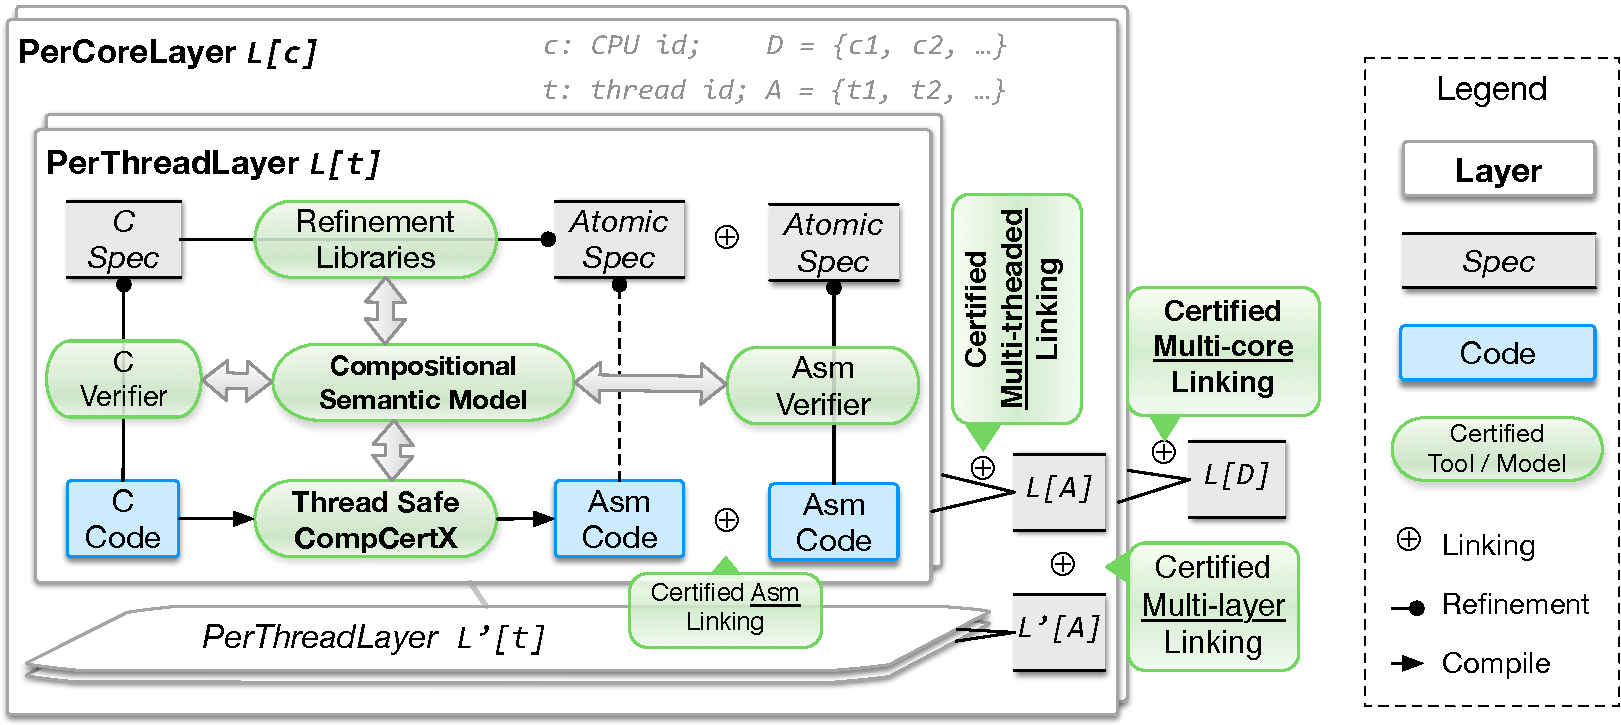
\includegraphics[scale=.45]{figs/tool_chain}
\caption{System architecture of the CCAL programming toolkit.}
\label{fig:toolchain}
\end{figure*}

\begin{table}
\begin{center}
\begin{footnotesize}
\renewcommand{\arraystretch}{1} 
\begin{tabular}{|c|c||c|c|}
\hline
Component & LOC & Component & LOC \\
\hline
\hline
Auxiliary library & 6,200 & Multilayer linking & 17,000 \\
\hline
C verifier & 2,200 & Multithread linking & 10,000 \\
\hline
Asm verifier & 800 & Multicore linking & 7,000 \\
\hline
Simulation library & 1,800 & Thread-safe CompCertX & 7,500\\
\hline
\end{tabular}
\end{footnotesize}
\end{center}
\caption{Lines of proofs in Coq for the toolkit.}
%\hrulefill
\label{table:toolkit}
\end{table}

We have implemented the CCAL toolkit (see
Fig. \ref{fig:toolchain}) in the Coq proof assistant. Table
\ref{table:toolkit} presents the number of lines (in Coq) for each component in Fig.~\ref{fig:toolchain}. The auxiliary library contains the common
tactics and lemmas for 64 bit integers, lists, maps, integer
arithmetic, {etc}.

\begin{table}
\begin{center}
\renewcommand{\arraystretch}{1.1}
\setlength{\tabcolsep}{0.3em}
\begin{tabular}{|c|c|c|c|c|c|c|}
\hline
 & \makecell{ C \& Asm \\Source} & Specification & \makecell{Invariant \\ Proof} & \makecell{C \& Asm \\Proof} & \makecell{Simulation \\ Proof} \\
%\cline{3-4}
% & Source & Specification & Invariant Proof & Proof & Proof  \\
\hline
Ticket lock & 74 & 615 & 1,080 & 1,173 & 2,296 \\
\hline
MCS lock & 287 & 1,569 & 2,299  &  1,899 & 3,049 \\
\hline
Sequential queue & 377 & 554 & 748 & 2,821& 3,647 \\
\hline
Shared queue &  20 & 107 & 190 & 171& 419\\
\hline
Yield/Sleep/Wakeup & 62 & 153 & 166 & 1,724 & 2,042 \\
\hline
Queuing lock & 112 & 255 & 992 & 328 & 464\\
\hline
\end{tabular}
\newline
\end{center}
\begin{flushright}
* Starvation proof for Ticket lock included: 980\\
** Starvation proof for MCS lock included: 2,455
\end{flushright}
\caption{Statistics for implemented components.}
\label{table:evaluation}
\hrulefill
\end{table}

\para{Case Studies}

To evaluate the framework itself, we have implemented, specified, and verified various
concurrent programs in the framework. Table \ref{table:evaluation} presents some of the
statistics with respect to the implemented components.
\ignore{ in terms of the number of lines of C \& assembly
source code, the number of layers used to specify and verify the module, the size of the
specification, and the number of lines
(in Coq) used to perform the invariant proof, code proof, and refinement proof, respectively.}
As for lock implementations,
their source code contains not only
the code of the associated functions,
but also the data structures and their initialization.
In addition to the top-level interface, the specification contains all the 
specifications used in the intermediate layers.
For both the ticket and MCS locks,
the simulation proof column
includes the proof of starvation freedom (about 1,500 lines) in addition to the correctness proof.
The gap between the underlying C implementation and the high-level specification of the locks
also contributes to the large proof size for these components.
For example, intermediate specification of the ticket lock uses an unbounded
integer for the ticket field,
while the implementation uses a binary integer
which wraps back to zero.
Similarly, the queue is represented as a logical list in the specification,
while it is implemented as a doubly linked list.

Our development is compositional. Both ticket  and MCS locks share the same
high-level atomic specifications (or strategies) shown in Sec.~\ref{sec:informal}.
Thus the lock implementations can be freely interchanged without affecting any proof
in the higher-level modules using locks. When implementing the shared queue library, we
also reuse the implementation and proof of the sequential queue library:
to implement the atomic queue object, we simply wrap the
sequential queue operations with lock acquire and release statements.
As shown in Table \ref{table:evaluation}, using verified lock modules to build
atomic objects such as shared queues is relatively simple and does not require
many lines of code.

Following the same philosophy, 
Gu et al. \cite{certikos-osdi16} has further extended our work with paging-based
dynamically allocated virtual
memory, device drivers with in-kernel interrupts, a synchronous inter-process
communication (IPC) protocol using the queuing lock, a shared-memory IPC protocol with
a shared page, and Intel hardware virtualization support;
our CCAL toolkit was used to produce the world's
first fully certified concurrent OS kernel
with fine-grained locking. 
\ignore{The entire kernel is reported to contain 6,500 lines
of C and x86 assembly code, and the verification effort for the concurrent kernel
is reported to be 2 person years.} 


\ignore{
To evaluate the framework itself, we have implemented, specified, and verified various
concurrent programs in the framework. Table \ref{table:evaluation} presents some of the
statistics with respect to the implemented components.
\ignore{ in terms of the number of lines of C \& assembly
source code, the number of layers used to specify and verify the module, the size of the
specification, and the number of lines
(in Coq) used to perform the invariant proof, code proof, and refinement proof, respectively.}
\ignore{The largest component is a thread linking refinement component. 
The LoC of multithread linking in Tab.~\ref{table:toolkit} only counts  
generic toolkit files. 
Instantiating them with our actual layer interface definitions which are described in 
Sect.~\ref{sec:multithreaded-layers} requires the refinement of the whole primitives 
in $\Lbthread[i]$ on CompCertX
and $\Lhthread[i][j]$ on Thread-safe CompCertX.
Therefore, the proof heavily relies on the size of layer interfaces.
In this sense, the proof size becomes big in our example because
$\Lbthread[i]$ or $\Lhthread[i][j]$ contains around 70 primitives, 
However, their proofs have redundant parts that can be further optimized 
and automated in the future.}

Lock implementations are  big parts in our examples. 
The first reason or this large LoC is the subtlety of busy waiting in the lock implementation 
(line 14 in Fig.~\ref{fig:exp:ticket_lock_example}). This requires us a large number of proofs to show 
 this loop
terminates within a bound (\ie, starvation-freedom). 
The other reason is mainly related to the strategy simulation 
that we have explained in Sec.~\ref{sec:informal}. 
Since our main goal is facilitating our toolkit for a large concurrent software system 
with scalability,  we have to make sure the the spinlock module provides
a general and simple interface.
This requires us to lift the low-level strategies (or specifications)
of two lock implementation to the same atomic interface (see Sec.~\ref{sec:informal}), which make proofs big.
Despite of this large LoC, however, the client of spinlocks can be verified over a simple interface
thanks to our toolkit.
\jieung{Will reduce and refine this paragraph again.}

\ignore{Their source code contains not only
the code of the associated functions,
but also the data structures and their initialization.
In addition to the top level interface, the specification contains all the 
specifications used in the intermediate layers.
For both the ticket and MCS locks,
the refinement proof column
includes the proof of starvation freedom (about 3,500 lines) in addition to the correctness proof.
The gap between the underlying C implementation and the high level specification of the locks
also contributes to the large proof size for these components.
For example, the intermediate specification of the ticket lock uses an unbounded
integer for the ticket field,
while the implementation uses a binary integer
which wraps back to zero.
Similarly, the queue is represented as a logical list in the specification,
while it is implemented as a doubly linked list.}

In addition to that, Our development is modular. 
Both ticket and MCS locks have the same
abstract specification,
thus the lock implementations can be freely interchanged without affecting any proof
in the higher-level modules using locks. When implementing the shared queue library, we
also reuse the implementation and proof of the sequential queue library:
to implement the atomic queue object, we simply wrap the
sequential queue operations with lock acquire and release.
As shown in Table \ref{table:evaluation}, using verified lock modules to build
atomic objects such as shared queues is relatively simple and does not require
many lines of code.
In addition, we can reuse the same lock verifications and specifications to verify other shared 
objects including a page allocation table.
In this sense, the large number in two lock components are reasonable trade-off
with all the benefits of our toolkits. 

Following the same philosophy, \citet{certikos-osdi16} has
further extended our work with paging-based dynamically allocated
virtual memory, device drivers with in-kernel interrupts, a
synchronous inter-process communication (IPC) protocol using the
queuing lock, a shared-memory IPC protocol with a shared page, and
Intel hardware virtualization support for simultaneously running
multiple virtual machines (one on each core); our CCAL toolkit was
used to produce the world's first fully certified concurrent OS kernel
with fine-grained locking.
\ignore{The entire kernel is reported to contain 6,500 lines
of C and x86 assembly code, and the verification effort for the concurrent kernel
is reported to be 2 person years.} }

\para{Performance Evaluation} 
\ignore{The verification should not by any means hinder the performance.
One benefit of the layered approach is that
concrete and highly optimized (and thus complex) implementations can be abstracted
into much simpler logical specifications that are easier to reason about.
In our toolkit, the verified source code (both C and assembly) are encoded as
abstract syntax trees in Coq, while CompCertX is written directly in
Coq. We then use Coq's extraction mechanism to produce a program which
compiles the C source code and outputs a single piece of assembly code
for the system. The resulting code is efficient.}
We have measured the performance
of the ticket lock on an Intel 4-Core i7-2600S (2.8GHz) processor with 16GB memory.
Initially, the ticket lock implementation incurred a latency of 87 CPU cycles in the
single core case.
After a short investigation, we found that we forgot to remove some function calls
to ``logical primitives'' used for manipulating ghost abstract states. After we removed
these extra null calls, the latency dropped down to only 35 CPU cycles.
%%%
Gu et al. \cite{certikos-osdi16} also presented performance
evaluations of their OS kernel built using CCAL.
They show that the MCS lock implementation scales better with more cores.
Additionally, they show that their kernel with fine-grained locking
performs significantly better than that with 
a big-kernel-lock implementation. The hypervisor performance is
also reported to be comparable to that of KVM.
